\documentclass[11pt,a4paper,titlepage]{article}

% Remove the .aux and .toc files if you switch languages
\usepackage[english]{babel}
%\usepackage[danish]{babel} % Danish hyphenation, headings, etc.

%\usepackage[utf8]{inputenc} % For Danish characters on Linux/Mac?
%\usepackage[latin1]{inputenc} % For Danish characters on Windos?

\usepackage{graphicx} % for the \includegraphics command
\usepackage{rotating}
\usepackage{booktabs} % for pretty tables

\usepackage{caption} % For better-looking figure captions
\renewcommand\captionfont{\slshape}

\usepackage{fancyhdr} % For custom page header/footer
\usepackage{longtable}
\usepackage{listings}
\usepackage{geometry}
\renewcommand{\arraystretch}{1.5}
\usepackage{tabulary}
\usepackage[newcommands]{ragged2e}
\geometry{left=2.5cm,right=2.5cm,top=2.5cm,bottom=2.5cm}

% Options for listings package
\lstset{
 language=Java,
 basicstyle=\sffamily, % it's either this or \ttfamily
 tabsize=4, % if your source code has tabs in it
 columns=fullflexible, % variable-width font
 showstringspaces=false, %Leaves spaces in strings blank
% emphstyle=,
}

% This demonstrates how to define custom commands.
\newcommand{\ex}[1]{\exists #1.\;}
\newcommand{\fa}[1]{\forall #1.\;}

\title{\huge{The Internet and Mobile Computing Laboratory Report}}
\author{IMCL}

\begin{document}

\maketitle
\tableofcontents

% European-style paragraph spacing. Note: must appear _after_ TOC
\setlength{\parindent}{0pt}
\setlength{\parskip}{1.8ex plus 0.5ex minus 0.2ex}

\clearpage

% This is where you set headers and footers. See the fancyhdr documentation for
% more details, especially for headers that are different on even- and
% odd-numbered pages (add the ``twoside'' optional argument to \documentclass.)
\pagestyle{fancy} % add header/footer from here on
\lhead{\slshape \leftmark} % Section name/number in left header
\chead{} % Blank center header
\rhead{} % Blank right header

\section{Themes in the IMCL Group}

The research of the IMCL group is mainly focused on 4 Themes : Smart sensing, wireless networks, mobile cloud computing, big data, and pervasive computing. Under these themes, we have a total of 19 research topics. The research themes and the corresponding research topics are shown in Fig. 1.

\begin{figure*}
\begin{center}
\includegraphics[angle=0,width=8cm,height=24cm]{Structure2.pdf}

\end{center}
\caption{} %The time intervals of received packets. .}
\label{fig:topics}
\end{figure*}


\textbf{1. Wireless Networks}

A heterogeneous wireless networking technology for seamless communication and mobility
Smart phones have taken the world by storm, with their global sales set to hit 1 billion by 2010.  On top of normal phone functions, a smart phone serves in an additional capacity as a mobile computing device. This marks a rapid shift in web surfing habits from the desktop to the mobile phone. In a parallel move, consumers want to access the Internet anytime, anywhere.  To make the Internet more mobile, we have developed a platform of heterogeneous advanced wireless networks known as ��HAWK��, which delivers an unprecedented level of mobility and coverage for Internet access that the mobile generation would love.

With this revolutionary technology in place, mobile users would roam smoothly and continuously as they hop across Wi-Fi, 2.5G and 3G cellular networks.  The transition is totally seamless and transparent, thanks to HAWK��s seamless handoff technology which dramatically speeds up the handoff process, allows the switching to occur automatically and makes intelligent decisions to adjust the quality of multimedia service to network capacity. As a result, users no longer lose connections and do not need to manually reconnect again while they are on the move, making their Internet access much smoother and more convenient, especially during Internet phone call or video conferencing.  While moving through the metropolitan cities, people can now enjoy their on-line games and the upcoming 2010 World Cup live broadcast seamlessly and continuously.

Furthermore, the HAWK uses advanced Wi-Fi meshes to link up hotspots, trying to extend Wi-Fi coverage beyond islands of broadband by filling the void in between.  Better still, it enables Wi-Fi access to penetrate even the most impossible locations, such as rough terrain or places with no fixed infrastructure.  Given its excellent reliability, this unique technology delivers unprecedented coverage of Wi-Fi for unbeatable online experience.  In the future, mobile users can enjoy at all times high quality, high speed, and unlimited broadband access wherever they go, at a higher rate than 3G.

In addition, we also focus on vehicular networks. We have developed vehicular networks based on software-defined network (SDN).


\textbf{2. Smart Sensing}

The objective of this theme is to realize efficient sensing, computing and communication in resource-constraint wireless and mobile networks for a wide range of applications such as wireless sensor network based structural health monitoring, human centric healthcare based on smart sensors, smartphone applications, localization systems, etc.

Figure \ref{fig:WNWSN} shows a research framework that covers the main topics we are interested. Please refer to the research topics under this theme for details.%The research topics are mainly focused on distributed computing in data-intensive and computation-complex applications; crowd souring,

\begin{figure}
	\centering
		\includegraphics[width=0.6\textwidth,height=.4\textwidth]{WNWSN.jpg}
	\caption{Research Framework of wireless networks and wireless sensor networks group}%The time intervals of received packets. .}
	\label{fig:WNWSN}
\end{figure}

\textbf{3. Mobile cloud computing}

The objective of this them is to design compute-intensive or data-intensive mobile applications by using cloud computing technology. is not trivial to develop compute-intensive applications on mobile devices with the aim of achieving low latency and energy consumption. It is also challenging to develop data intensive mobile applications, since it re-quires effective ways to process and analyze the big data from the mobile applications. To solve these two challenges, we have dedicated many efforts in developing algorithms and mechanisms at different technical layers such as resource management, data management, computation scheduling and programming abstraction.

Figure \ref{fig:MCC} shows a research framework that covers the main topics in the field of mobile cloud computing. The topics are classified into various system layers: resource management, computation and data management, programmng models and applications. Note that the resources in mobile cloud environment consist of the networking, computation and storages from mobile nodes, cloudlets distributed at the network edge and centralized data centers on the Internet. At resource management layer, the main goal is to abstract the resources from various distributed hosts, and provision them as services to consumers. The research issues at this layer may be quite different depending on specific system models and objectives. For example, in ad hoc based mobile cloud model, one issue is to design effective mechanism to incentive more peers to participate into the system and share their computing resources.


\begin{figure}
	\centering
		\includegraphics[width=0.6\textwidth,height=.4\textwidth]{MCCFramework.jpg}
	\caption{Research framework of mobile cloud computing} %The time intervals of received packets. .}
	\label{fig:MCC}
\end{figure}

On the topic of resource management layer, we are facing a few issues related to computation and data management. One hot topic studied extensively recently is computation partitioning, i.e., to decide for mobile devices which parts of application should be computed on the mobile devices and which parts should be offloaded onto cloud, such that certain objective like computation time and energy consumption is optimized. Highly associated with computation partitioning, another issue is computation scheduling of the off-loadings from mobile users onto the data center resources.

Besides computation related research, there exist continuous efforts on the data centric research in mobile cloud, which is named as data management in our framework. The re-search area assumes a smart mobile cloud system that is able to collect, analyze, store (place), and deliver the data intelligently and efficiently. To be specific, data collection focuses on how to aggregate/fuse and then gather the data from multiple mobile devices to the centralized cloud in an energy efficient way. Data analysis particularly focuses on the design of computing platforms for data processing, and algorithms for data analysis. Data placement and data delivery aims to provide good quality data services for the end users.

At programm model layer, much research efforts have been dedicated on the design of easy-to-use programming models for develop various mobile cloud applications. Due to the inherent data intensive property of most mobile cloud applications, one research issue lies on how to design easy-to-use programming models and interfaces for big data application developers. At application layer, researchers are focusing on development of novel applications re-lying on mobile cloud system technologies. Some popular applications that inherently need to leverage the cloud computing are mobile interactive perception application, mobile augmented reality, community sensing applications and so on.

The right side of the framework lists four interests that could be focused by researchers: performance, economics, privacy and security. The four interests are classified from the perspective of research objectives, and involve the techniques across all the layers. The performance related topics include the performance monitoring, diagnosis and optimization. The economics cover the topics of pricing models and auction models, and monetary cost optimization.

Our research focuses on a few but not all topics in the framework. First, we have dedicated most efforts on the performance optimization specifically at the layer of computation and data management. Specifically we focus on the issue of computation partitioning and scheduling, and data placement. Second, we also have done some works on programming models for big data process. We focus on developing a framework for integrating existing big data programming models using a unified interface. Third, we have been developing mobile multimedia applications by mobile cloud technologies. One novel application we focus on is touch free HCI on smart phones. We have designed live video based gesture recognition algorithms, and aim to optimize the performance on smart phones.



\textbf{3. Big Data}

The objective of this theme is to provide methods and mechanisms for collecting, organizing, processing and analyzing huge volumes of data. With the capability of analyzing big data, we can uncover hidden patterns, unknown correlations and other useful information to make better decisions. It is challenging to design models and algorithms for parallel data processing and data mining in various application areas. Meanwhile, since we need to utilize cloud resources effectively in processing and analyzing big data, it is important to ensure the performance of data-intensive applications in cloud environment. In face of these challenges, we make many efforts in designing algorithms and mechanisms at different technical layers such as data analysis, data processing, data management, etc.

As shown in Fig. \ref{fig:BD}, our research framework covers the main topics in the field of big data analytics. The topics are classified into various system layers. These layers differ in function, system level, specific interface, and the extent of interaction with users. In the hierarchical structure of this framework, three primary layers are defined for decision-making processes, including data processing, data analysis and application layers.

\begin{figure}
	\centering		 \includegraphics[height=.6\textwidth]{BD.pdf}
	\caption{Research Framework of Big Data Group}%The time intervals of received packets. .}
	\label{fig:BD}
\end{figure}




\textbf{4. Pervasive Computing}

The objective of this theme is to develop theories/methodologies for building high performance pervasive computing systems, and ease its development/testing by providing various tools. Among pervasive computing, we currently focus on two important applications, distributed MEMS (micro-electro-mechanical systems), and searching and browsing cyber-physical objects. For the former one, we aim to provide programming support and design efficient and effective algorithms for distributed MEMS. And for the latter one, we aim to develop efficient approaches for the browsing and searching the objects in cyber-physical systems. We believe that our research will make valuable contributions to the pervasive computing and the internet of things, and make people's life easier, healthier, and happier.

Figure~\ref{fig:MEMS} shows a research framework of programming distributed MEMS. There are three aspects for programming distributed MEMS, named programming principle, programming paradigm, and supported features. The programming principle defined the view of programmers to the MEMS, either ensemble-based or individual node-based. The latter follows the traditional distributed development, considering the distribution of data and function in individual nodes and communication among them. On the contrast, the ensemble-based way considers all the individual nodes as a whole and specifies the common rules for them to achieve objectives. All the underlying data distribution and communication are left to the system implementation.  For the programming paradigm, the application development can be based on declarative languages or imperative languages. Finally, the sup-ported features include scalability, fault-tolerance, real-time, feedback control, etc. Real-time support is our current focus, and can be investigated on the topics on the time specification, time estimation, scheduling, and real-time control

\begin{figure}
	\centering		 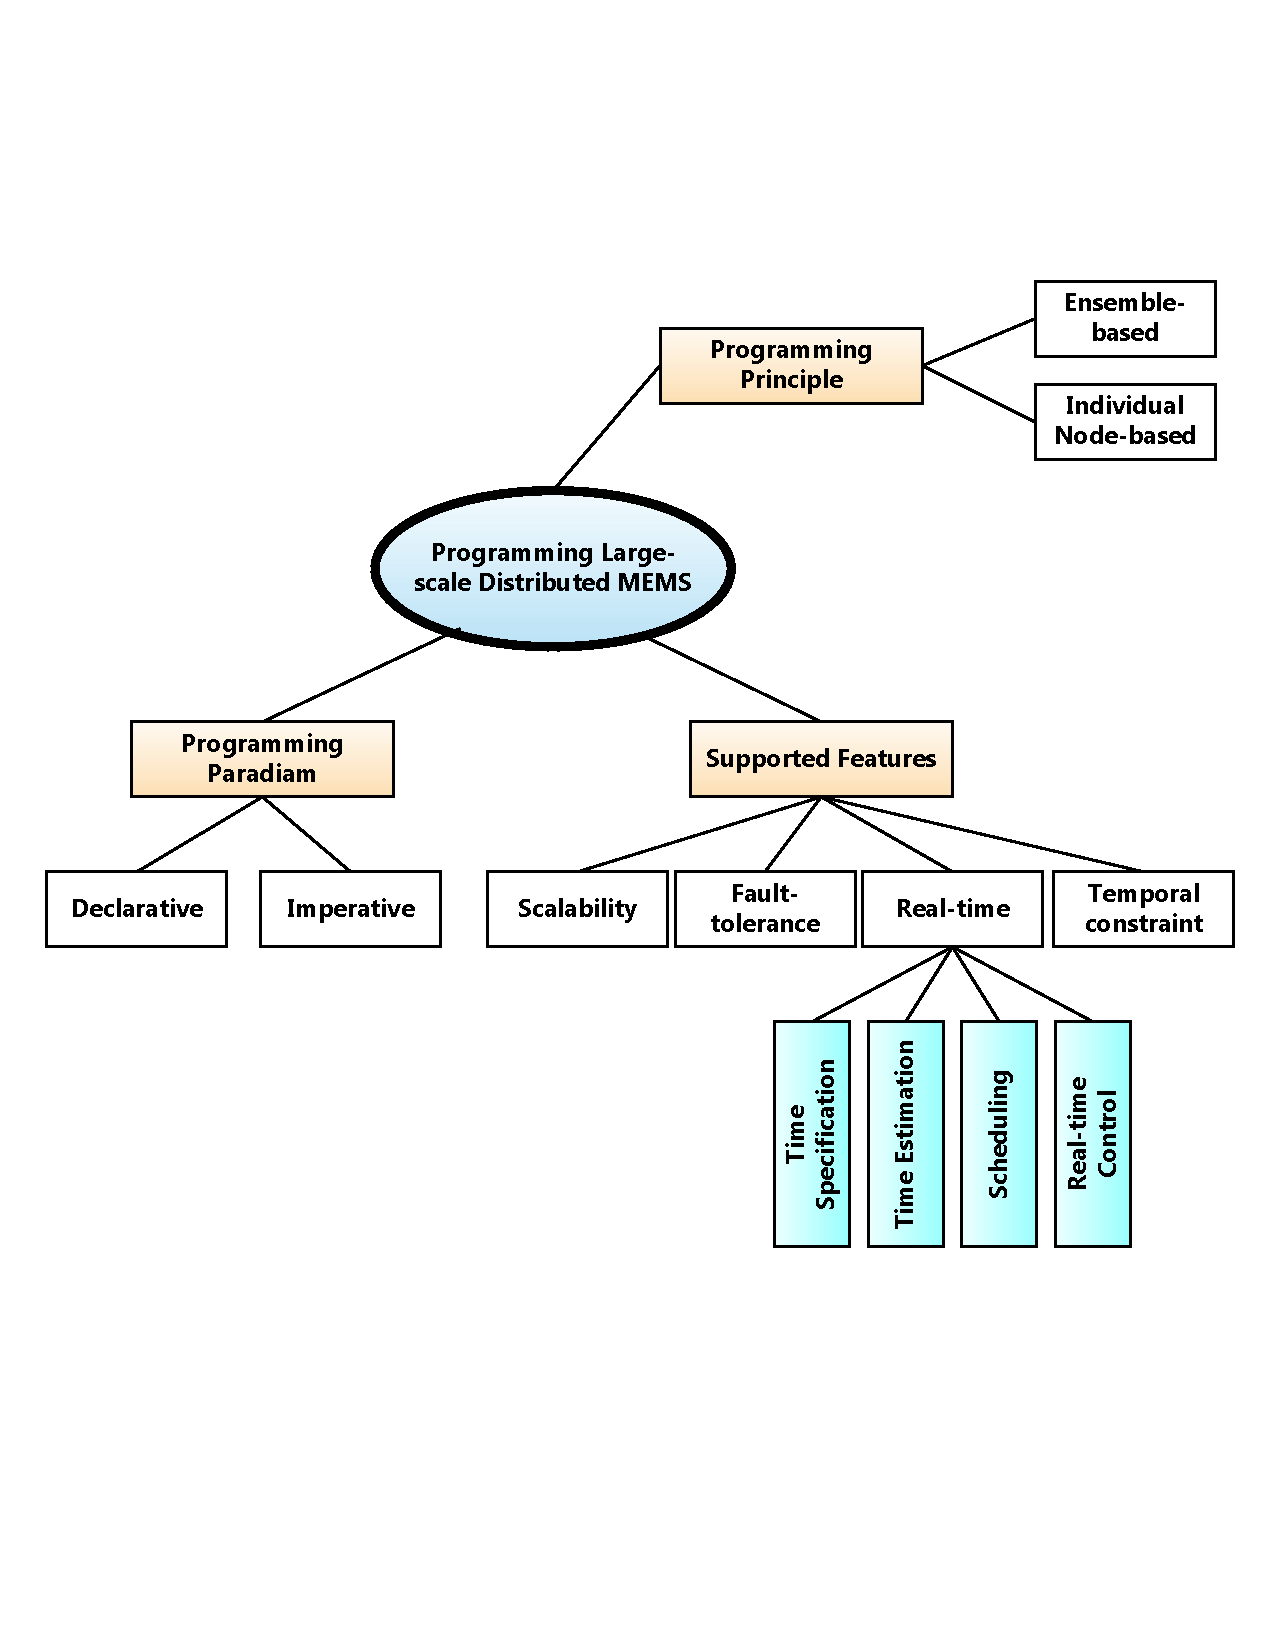
\includegraphics[height=.6\textwidth]{MEMS.pdf}
	\caption{Research Framework of Programming Support for Distributed MEMS}%The time intervals of received packets. .}
	\label{fig:MEMS}
\end{figure}

Figure \ref{fig:USBF} shows a research framework that covers the main topics of searching and browsing cyber-physical objects.
The topics are classified into five layers: information collection, communication and networking, modeling, programming support, and application. Information collection layer is responsible for collecting information from objects in the cyber world and in the physical world. It needs to conduct identification, localization, spatio/temporal correlation, and social correlation to different objects. Communication and network layer is responsible for connect different objects into a network for the ease of searching and browsing. The major functions include access, rout-ing, caching, service handoff, etc. On the top of it, proper modeling approaches are needed for the operation and development in such systems. The modeling need to cover the objects, its at-tributes, relationship among objects, services, and behaviors. Based on this model,  some key programming supports are provided,  including storage management, index building, query matching, result ranking, relation detection and inference, to the user for the ease of the application development, object searching and object browsing.

\begin{figure}
	\centering		 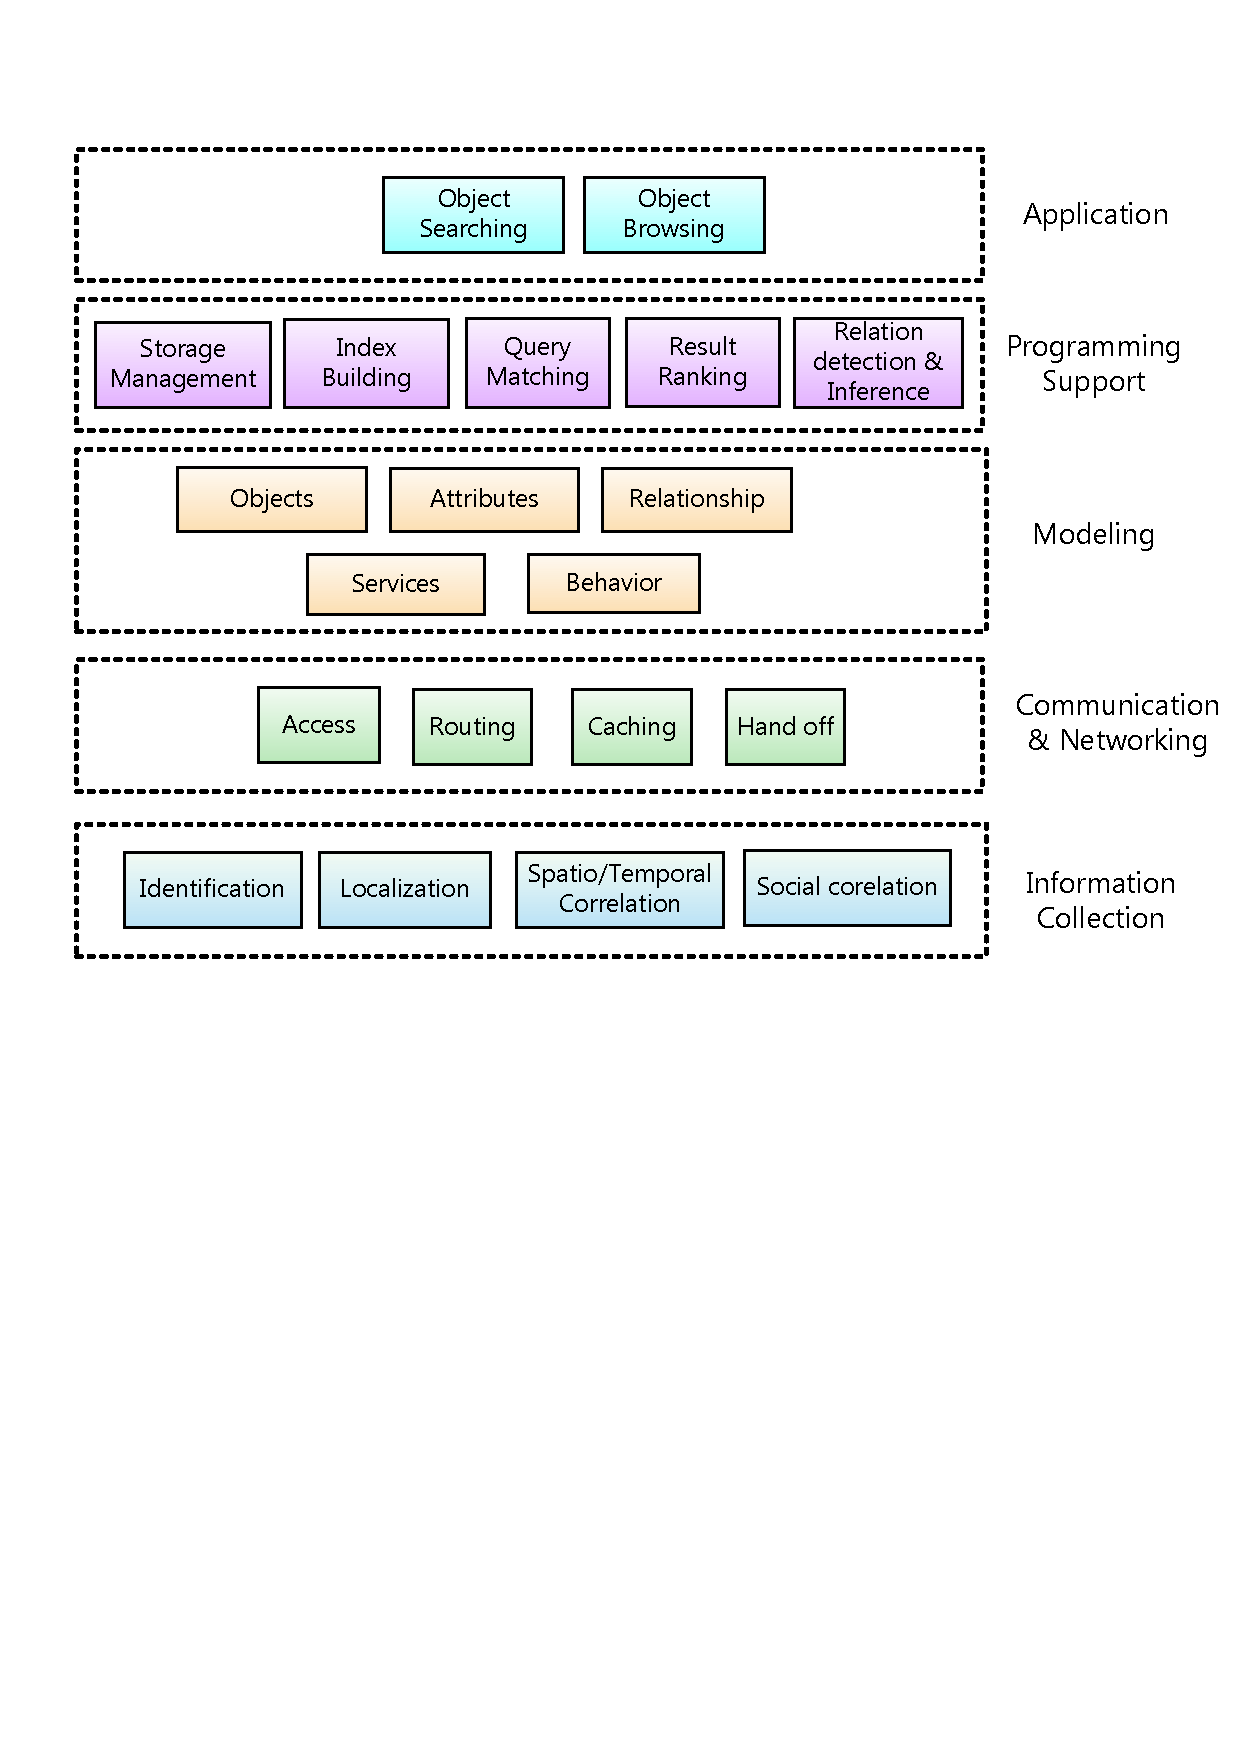
\includegraphics[height=.6\textwidth]{USBF.pdf}
	\caption{Research Framework of Searching and Browsing Cyber-physical Objects}%The time intervals of received packets. .}
	\label{fig:USBF}
\end{figure}

\section{The Topics}

Under the 4 research themes, we have a total of 18 topics.
%
%Fig. \ref{fig:topics} shows the topics under different themes and the group members involved in each research topic.
%
%
%
%\begin{figure*}[htbp]
%\begin{center}
%\includegraphics[angle=0,width=8cm,height=24cm]{Structure.pdf}
%\end{center}
%%\caption{Research themes and topics} %The time intervals of received packets. .}
%	\label{fig:topics}
%\end{figure*}



\subsection{S-Helmet}

Introduction:

Although the safety performance of the high-risk construction industry in Hong Kong has continued to improve, construction site accidents still accounted for nearly one-fifth of all the industrial accidents in Hong Kong. Safety policies and standards have proven to be less than completely reliable in many cases due to the complicated and dynamic environment in construction sites. ��Fall of person from height�� and ��Striking against or struck by moving or stationary objects such as construction hoist and tower crane�� are the top two killers in the construction industry.  It would be highly desirable to have a proactive safety management system able to continuously monitor workers�� locations and automatically issue warning alarm.

We propose to develop such a system for construction safety, called s-Helmet, based on the real-time localization technique we have designed.  In s-Helmet, wireless tags are attached to the safety helmets of workers and moving objects to track their locations in real time. When a worker is moving near danger zones (e.g. edge of the working platform, close to moving objects or electric discharge, etc.), the helmet will automatically issue an alarm to the worker as well as the construction site coordinators. We believe this system can effectively help to avoid the construction accidents and has great impact on the construction safety in Hong Kong. We summarize the functions of the S-Helmet.

\begin{enumerate}
  \item To prevent the occurrence of some dangers (e.g. fall of person from height and striking against a moving objects).
  \item To provide the real-time information for construction site management.
  \item To give real-time healthy information of the construction workers.
\end{enumerate}


Objective:

In this demo, we mainly have three research objectives:

\begin{enumerate}
  \item To design optimal MAC and routing protocol which is about to realize fast locali-zation of NanoLoc tags.
  \item To design a scheme to address the localization error caused by non-line of sight problem to the NanoLoc tags.
  \item To design energy efficient scheme to maximize the network lifetime of the tags.
\end{enumerate}

\subsection{Walk-Safe: A pedestrian safety application for mobilephone uers}

Introduction
Recently, a research trend is focus on the effect of mobile phones on pedestrian safety due to wide usage of phones. Some studies demonstrate that mobile phone users exhibited more unsafe behavior than common people. For instance, the users are distracted and less aware of situation ahead, leading to falling and bumping injuries. Meanwhile, a number of research papers demonstrate some smart phone applications to enhance the pedestrian safety. Majority of them focus on utilizing the camera to help pedestrian be aware of unsafe condition. Though those applications can bring some benefit to users, they will bring great impact to battery-life due to utilizing high power consumption camera module. Thus, the energy drain issue has become a main drawback. To protect pedestrian and alleviate the battery drain issue, we have designed this safety application WalkSafe with a different approach. Instead of utilizing camera module, our system exploits an ultrasonic sensor attached into the mobile phone. Through analyzing the distance data collected from ultrasonic sensor, our system could help pedestrian avoid accident by notifying users peril ahead.
However, it presents several challenges in our work. For example, in order to alleviate the energy drain problem, a sophisticated power management policy should be proposed. On the other hand, a vibrating mobile phone produces noise and large variation in the readings from sensors due to the footfall, which should be filter out before being able to utilizing them. Furthermore, frequent meaningless disturbance tends to make users annoyed. Thus, we should figure out a way to reduce the disturbance to users. All these challenges are the barriers to build a robust pedestrian protect system under real-world conditions.
Consequently, we have set up the following requirements for our system: 1) Walker should be capable of real-time detection and notify users in a timely manner. 2) Walker should reduce the influence on mobile phone, including the battery consumption and system performance. 3) Walker should bring good user experience for users, reducing the meaningless disturbance time.

Objective
In this topic, we mainly have the following research objectives.
1.     Provide a safety application for pedestrian mobile phone users.

2.     Design a power management policy making the application more battery-friendly.

3.     Design a context-aware technology that minimizing the disturbance to user.

4.     Propose a method to reduce the noise in the data collected from sensors. 
\subsection{Smart Cushion}

Sitting posture particularly poor posture greatly influences one's health and in-creases the risk of developing upper limb and neck disorder. Therefore, it is greatly desirable to develop a system that recognise user��s sitting postures, and then generate alerts for poor postures. Current solutions for sitting posture recognition either use intrusive wearable/visual sensors or rely on expensive high-resolution pressure sensor array, and thus limiting their usability and widespread deployment.
The objective of this project is to develop a sitting posture recognition system that is accurate, non-intrusive and low-cost. In specific, the proposed system is able to accurately infer a set of common sitting postures based on a few number of pres-sure sensors deployed on the seat cushion. This project introduces two main innovations. First, we propose a set of user-invariant and distinctive features to model sitting posture, which improves the recognition accuracy. Second, we conduct a systematic research on the optimal sensor placement with respect to different sitting posture sets, achieving the balance between system accuracy and cost.

\input{../SmartSensing/TOpics-LR}
\subsection{Traffic Signal Schedule Estimation Using Smartphone}

Problem:

Generally, the problem is to estimate the traffic signal schedule information using smartphones.

Formally, we define the problem as: Given: a set of traffic lights and their locations, a set of vehicle traces including, accelerations and locations; Assume: traffic signal schedule model ( parameterized by Tc and Tg ) on-board smartphone is relatively static to the vehicle; Objective: estimate traffic signal schedule model parameters, Tc and Tg for accuracy within 1s.

Motivation:

Traffic light is a key element in everyday traffic management. Drivers can make better decision including velocity alteration and road chosen if he/she can acquire the upcoming traffic light in-formation, so that a considerable quantity of fuels can be saved.

It is very challenging to accurately recognize the traffic light, due to the complexity of the real world traffic scene. In particular, for traffic light, not only the shapes and position alters, but also the basic construction differs, including the with/without remaining time notification, traffic light for one way, two way or three ways.
Existing work focused on solutions using cameras. These methods have the several constrains. Firstly, they require each vehicle equipped with specific devices to capture videos and do analysis. Secondly, vision-based method is very hard to be robust to the environment changing. For in-stance, vision based algorithms will be influence a lot in rainy or snowy days.

Solution:

We proposed a two-stage traffic signal schedule estimation approach. At the first stage, on-board smartphone detects vehicle event of acceleration or deceleration based on the accelerometer sensing data and report the event to a server. The server, at the second stage, collects a set of such events to estimate the traffic signal changing sequence. The moment with rapidly in-creasing number of accelerating vehicle is marked as the time red signal changed to green one and vice versa for green to red signal changing.

Result:

We have conducted experiment to evaluate the performance of iTraSig. The overall architecture of iTraSig involves two main components which are implemented on different platform, respectively, smartphone and central server. Mainly focused on testing the function of event detection, we did experiments in different types of real vehicle, providing comparisons between the ground truth and our detected results. On the server side, we did two simulations showing estimated resulted in various scales. A simulation of single intersection is conducted to show the feasibility and effectiveness of the algorithm. Moreover, a multi-intersection simulation is done to show the performance of iTraSig in terms of estimation time in diversity of traffic flows.

%
\subsection{SDN based Vehicular Network}

With the advancement of wireless communication and embedded technology, vehicles nowadays are becoming a powerful sensing, computing and communication platform. Vehicles can be connected to the Internet and ambient vehicles using wireless networks. However, challenges remain for developing practical and large-scale real world vehicular network applications. For example, the heterogeneity of wireless technology (3G/LTE, Wi-Fi, DSRC/IEEE 802.11p) used in vehicle communications has caused network fragmentation due to the difficulty in integration. In addition, the decentralized vehicle-to-vehicle (V2V) routing protocols are fragile to the highly dynamic vehicle mobility. The emerging software defined networking (SDN) technology provides new insights and alternative approaches to develop solutions of vehicular networks that can tackle the aforementioned problems. SDN has attracted great attention from both academia and industry in recent years. The separation of data plane and control plane and the employment of ��logically centralized�� management architecture can not only simplify the network management but also bring new services to the applications.

Currently, research on SDN mostly focuses on rethinking and redesigning wired network architectures, but not for wireless networks. In this project, being the first, we investigate the requirements and challenging issues in applying SDN to developing high-performance vehicular networks. More specifically, we design a framework to manage heterogeneous vehicular networks to improve the performance in multi-hop routing and inter-network flow switching and application-specific dataflow transmission. The framework is based on the abstraction and integration of the underlying heterogeneous wireless networks and provides a logically centralized way to greatly simplify the design of vehicular network management. As one of the key components, the framework consists of mechanisms and algorithms for collecting and maintaining the states of individual vehicles, which will be used by the SDN control plane to perform centralized optimization of routing and inter-network switching. In doing this, we will also address the challenging issues of network failures and recovery, vehicle mobility prediction and cooperative state updating. We will evaluate the effectiveness and performance of the proposed framework via simulation. We will also develop some demo applications based on the prototype.

This topic will make significant contributions to vehicular network and software-defined networks. This is the first project that utilizes SDN to solve data transmission problems for vehicular networks. The output of this project can help vehicular networks to be applied at large scale. Companies with large number of vehicles like logistic companies and taxi companies will benefit from it.

Our objective is 

\begin{enumerate}
  \item To study and identify the new requirements and issues of developing advanced vehicular applications.
  \item To propose and design the SDN based heterogeneous communication framework. The framework includes algorithms of inter-vehicular communication, inter-network integration and adaptive protocol utilization, with scalability and reliability.
  \item To evaluate the effectiveness and performance of the proposed mechanisms and algorithms through theoretical analysis and simulations.
  \item To build a test-bed and implement the proposed communication framework with mechanisms and algorithms, and develop example applications with demonstrations.
\end{enumerate}


%
%
%
\subsection{Intelligent Transportation System Demo}

We have a platform to demonstrate our existing research results in intelligent transportation systems (ITS), which include the following research topics:

\begin{enumerate}
  \item WSN-assisted collision avoidance
  \item Demand-oriented intelligent traffic light control
  \item WSN-assisted tracking system
  \item Middlware for ITS
\end{enumerate}

The platform must be reliable and stable during the show. The previous implementation was based on the now obsolete and unmaintained TinyOS 1.x so these programs are gradually being ported to TinyOS 2.x for the sake of long-term benefit. We have already ported the following TinyOS 1.x applications:

\begin{enumerate}
  \item The TinyOS application running on each car
  \item The TinyOS application running on the traffic lights
  \item The Java application running on the gateway PC
\end{enumerate}

From the system architecture perspective, the platform can be divided into several layers from lowest to highest, including:

\begin{enumerate}
  \item Hardware and control: this layer includes the actual hardware boards which drive the demo cars, control the traffic lights and send feedbacks through UART
  \item Reliable wireless communication layer: this layer includes all the wireless sensor nodes. All sensor nodes communicate with the hardware boards via UART.
  \item Application layer: this layer includes all the Java applications running on the PC which handles traffic light control.
\end{enumerate}

The reliable communication layer is the heart of our platform because this is the part which ensures the correctness of our demo. To achieve a high degree of reliability, we have two mechanisms:

\begin{enumerate}
  \item Wireless link layer acknowledgement: each time when a packet is from one sensor node to another, the packet acknowledgement module is enabled with a maximum of 128 re-tranmission to ensure the messages will be reliably delivered.
  \item PC-to-node transport layer acknowledgement: in the transport layer, every time when an application sends a control command to the sensor network, the acknowledged packet will be sent back to the application. Then, on the application side, such information is used to determine if a command is lost or not. We have an application layer command check which runs as a background thread and periodically checks the commands sent. When the thread finds a command is sent but the acknowledged packet does not come back within the timeout, it will re-send the command.
\end{enumerate}




\subsection{SDN based Vehicular Network}

With the advancement of wireless communication and embedded technology, vehicles nowadays are becoming a powerful sensing, computing and communication platform. Vehicles can be connected to the Internet and ambient vehicles using wireless networks. However, challenges remain for developing practical and large-scale real world vehicular network applications. For example, the heterogeneity of wireless technology (3G/LTE, Wi-Fi, DSRC/IEEE 802.11p) used in vehicle communications has caused network fragmentation due to the difficulty in integration. In addition, the decentralized vehicle-to-vehicle (V2V) routing protocols are fragile to the highly dynamic vehicle mobility. The emerging software defined networking (SDN) technology provides new insights and alternative approaches to develop solutions of vehicular networks that can tackle the aforementioned problems. SDN has attracted great attention from both academia and industry in recent years. The separation of data plane and control plane and the employment of ��logically centralized�� management architecture can not only simplify the network management but also bring new services to the applications.

Currently, research on SDN mostly focuses on rethinking and redesigning wired network architectures, but not for wireless networks. In this project, being the first, we investigate the requirements and challenging issues in applying SDN to developing high-performance vehicular networks. More specifically, we design a framework to manage heterogeneous vehicular networks to improve the performance in multi-hop routing and inter-network flow switching and application-specific dataflow transmission. The framework is based on the abstraction and integration of the underlying heterogeneous wireless networks and provides a logically centralized way to greatly simplify the design of vehicular network management. As one of the key components, the framework consists of mechanisms and algorithms for collecting and maintaining the states of individual vehicles, which will be used by the SDN control plane to perform centralized optimization of routing and inter-network switching. In doing this, we will also address the challenging issues of network failures and recovery, vehicle mobility prediction and cooperative state updating. We will evaluate the effectiveness and performance of the proposed framework via simulation. We will also develop some demo applications based on the prototype.

This topic will make significant contributions to vehicular network and software-defined networks. This is the first project that utilizes SDN to solve data transmission problems for vehicular networks. The output of this project can help vehicular networks to be applied at large scale. Companies with large number of vehicles like logistic companies and taxi companies will benefit from it.

Our objective is 

\begin{enumerate}
  \item To study and identify the new requirements and issues of developing advanced vehicular applications.
  \item To propose and design the SDN based heterogeneous communication framework. The framework includes algorithms of inter-vehicular communication, inter-network integration and adaptive protocol utilization, with scalability and reliability.
  \item To evaluate the effectiveness and performance of the proposed mechanisms and algorithms through theoretical analysis and simulations.
  \item To build a test-bed and implement the proposed communication framework with mechanisms and algorithms, and develop example applications with demonstrations.
\end{enumerate}



\subsection{Intelligent Transportation System Demo}

We have a platform to demonstrate our existing research results in intelligent transportation systems (ITS), which include the following research topics:

\begin{enumerate}
  \item WSN-assisted collision avoidance
  \item Demand-oriented intelligent traffic light control
  \item WSN-assisted tracking system
  \item Middlware for ITS
\end{enumerate}

The platform must be reliable and stable during the show. The previous implementation was based on the now obsolete and unmaintained TinyOS 1.x so these programs are gradually being ported to TinyOS 2.x for the sake of long-term benefit. We have already ported the following TinyOS 1.x applications:

\begin{enumerate}
  \item The TinyOS application running on each car
  \item The TinyOS application running on the traffic lights
  \item The Java application running on the gateway PC
\end{enumerate}

From the system architecture perspective, the platform can be divided into several layers from lowest to highest, including:

\begin{enumerate}
  \item Hardware and control: this layer includes the actual hardware boards which drive the demo cars, control the traffic lights and send feedbacks through UART
  \item Reliable wireless communication layer: this layer includes all the wireless sensor nodes. All sensor nodes communicate with the hardware boards via UART.
  \item Application layer: this layer includes all the Java applications running on the PC which handles traffic light control.
\end{enumerate}

The reliable communication layer is the heart of our platform because this is the part which ensures the correctness of our demo. To achieve a high degree of reliability, we have two mechanisms:

\begin{enumerate}
  \item Wireless link layer acknowledgement: each time when a packet is from one sensor node to another, the packet acknowledgement module is enabled with a maximum of 128 re-tranmission to ensure the messages will be reliably delivered.
  \item PC-to-node transport layer acknowledgement: in the transport layer, every time when an application sends a control command to the sensor network, the acknowledged packet will be sent back to the application. Then, on the application side, such information is used to determine if a command is lost or not. We have an application layer command check which runs as a background thread and periodically checks the commands sent. When the thread finds a command is sent but the acknowledged packet does not come back within the timeout, it will re-send the command.
\end{enumerate}



\subsection{Computation Partitioning}

On this topic, we are going to implement a platform for developing next generation mobile applications by leveraging cloud computing technologies, i.e., by partitioning the computations of applications between mobile devices and the cloud, so we can create applications that far exceed traditional mobile device capabilities. For the applications running on the platform, we aim to achieve adaptive and elastic execution between the mobile devices and the cloud. This is motivated by the fact that many mobile devices like the iPhone have been equipped with various kinds of sensors and multimedia capabilities. We foresee that a lot of new mobile applications such as multimedia applications, object recognition, location-based social networks and augmented reality, will become highly demanded. By offloading the computation to the cloud, these advanced mobile applications which could not be accommodated before due to the lack of significant computing capability and energy power of mobile devices, will be enabled and enjoyed by mobile users.

This project will have essential benefits and long term impact to the mobile ecosystem. First, the platform is designed in particular for the application providers. It provides programming interfaces and runtime support for application providers to develop and deploy diverse varieties of advanced mobile applications. Particularly, in the programming phase, the developers write the application logic by using the APIs provided by us; while in the runtime phase, our platform is responsible for the partitioning of application functionalities between mobile and cloud side. The partitioning is done according to the available computing and network resources in the environment, and the performance requirements. By using our platform, the developers only need to focus on the application logic, while do not care about the partitioning of the functionalities.

Second, the platform will bring business opportunities for cloud providers as well as application developers. The application developers can make profits by quickly developing and selling various intelligent mobile applications on the platform, while the cloud resource providers can make profit by provisioning computation resources to accommodate the partitioned mobile applications.

The platform provides programming and deployment services for application providers, and run time support for the partitioned execution of application between mobile and cloud. In programming phase, the developer writes the application using certain programming abstraction and interfaces. In our platform, we are going to provide dataflow graph abstraction for developers to write the application logic. In this model, the application is composed a set of modules which may have data dependence among each other. The program code from application providers will be mapped into two cop-ies by our platform compiler. One copy is to be executed on the cloud virtual machines. The other one is to be executed on the mobile device.

In deployment phase, the developers can conveniently deploy the applications using our graphical user interface. The platform has a special storage component, called Application Models Warehouses, to store both two copies of the application code. When the users install the applications, the copy of mobile code will be downloaded onto the end users' devices.

The objective of this work includes:

1). To develop a platform for providing computation partitioning as a service in cloud environ-ments. By developing the platform, we will eventually deliver tools and software at both cloud and mobile side to provide programming and runtime support for application developers;

2). To develop a set of applications based on the platform with demonstration, and validate the performance with large test cases;

3). To research and validate the business models from perspectives of various stakeholders involved in the platform, i.e., mobile users, application developers and cloud providers.



\subsection{Service Placement}

The existing MCC model that enables the service provisioning directly from large centralized Internet data centers inherently incurs relatively high latency. Researchers point that the WAN latency could be as high as tens of milliseconds even when the users connect to the closest Internet data center. The latency may meet the requirement of most applications such as web browsing, but can yield bad usability/user experience for latency sensitive application such as high quality video streaming, mobile gaming, augmented reality and so on. To solve the problem, a lot of research works propose to add another abstraction tier between mobile users and centralized data centers.

We study the service placement problem in the 3-tier hierarchical system model (cloud-cloudlets-mobile users), in which the mobile users and cloudlets are geographically distributed. We have a set of services from the application provider to be placed on the cloudlets. The ideal case is that each user's demanding service is placed onto the cloudlet that is in the user's proximity. However, there are two possible cases that the users' demands are serviced from other cloudlets far away or the centralized cloud. The first case is that the users in proximity of the cloudlet may demand highly diverse services. However, placing all the demanded services onto the same cloudlet is not possible due to its storage capacity. Another case is we consider the compute capacity of cloudlets, and the load demands by mobile users from the cloudlet's proximity may exceed the cloudlet's capacity. Therefore, we face one basic problem which is to place a set of services onto cloudlets, and dispatch users' demands to the middle-tier cloudlets and the upper-tier cloud, such that the average latency of all the demands are minimized, while the capacity constraints of cloudlets are satisfied.

We further extend the service placement problem by considering the resource cost of the application provider. The resource cost of the application provider includes resource usages on the centralized cloud and distributed cloudlets. In particular, the cost on each cloudlet consists of the cost used to store the data associated with the placed services, and the compute cost which varies depending on the loads dispatched to the cloudlet. The cost on the cloud mainly includes the compute cost of the loads dispatched to the cloud. To ex-plain the resource cost of cloudlets, we envision two practical deployment settings of the cloudlets. One is that the cloudlets are deployed by wireless operators within the wireless access networks. Another is that cloud providers co-locate cloud resources in wireless ac-cess networks through co-location agreement with wireless operators. Throughout our pa-per, we name the party who provides cloudlet resources, e.g., the wireless operator in the former case or the cloud provider in the latter case, as the cloudlet provider. In real world, the cloudlets are from different cloudlet providers which may have various prices for the storage/compute resources. Besides the one-shot resource cost, we also consider additional cost incurred by the placement transition over two successive time slots. This is due to the fact that the services placed on cloudlets can be taken as replicas from the cloud. Placing new replicas on the cloudlet brings data transmission and thus bandwidths cost from the cloud to cloudlets. The extended service placement problem aims to balance the tradeoff between the operational cost and the average latency. The details of the problem description is as follows. 
\subsection{Resource Prediction}

The objective of this topic is to provision the resource for cloud services under the consideration of maximum the system utilization and users' cost. To solve the problem, two steps should be taken. First, we should predict the resource demand of cloud services accurately. Second, we should allocate appropriate resources to the given jobs. As is shown in Google workload trace published in 2011, the resource request is made manually. However, almost 60\% of the total jobs in the workload was killed by pro-grammers, which made a considerably CPU waste. What's more, some actual applications was delayed by resource contention. The average utilization of machines in the cluster is under 30\%. The real used resource is less than half of the resource request.

Consequently, resource prediction and resource allocation policies should be considered. Few works consider the resource provisioning problem on SaaS level, which actually is something of value. With a good resource prediction, one can save the cost for scheduling and migration. As I known, HP lab has done some work on the resource prediction for MapReduce services. However, their algorithm only considers the linear situation and ignores the communication between map and reduce tasks. Traditional resource prediction and scheduling policies only considers the homogeneous environment or workloads. How-ever, the workloads in the cloud computing environments has more diversity and heterogeneity. There are more challenges for resource provisioning for cloud services.

Three challenges exist to solve the problem. The first one is how to accurately modeling the workload. Maybe we can use the queuing theory to profile the arriving time, execution time, waiting time for a job.  The second one is how can be predict the resource demand as a vector other than a single value. We can try to solve the problem using newly multi-target prediction. The feasibility and accuracy should be tested and decided. The third one is how to determine the VM composition according to the resource demand. We can use integer optimization to solve the problem. I will develop a more accurate and light weighted model for resource prediction.



\subsection{Performance Management for Big Data Applications in Mobile Cloud Computing}

In mobile computing environment, the computation intensive and data intensive applications usually lead to unsatisfactory performance on resource limited mobile devices. As a new paradigm, cloud computing can enhance computing and storage capabilities of mobile devices for big data applications. The basic idea of computation offloading is to move the task execution from mobile devices to cloud infrastructures, which have clusters with faster processing speed.

Mobile computation and data offloading has been regarded as a research focus by researchers in recent years. The existing work on this problem differs in their cost-benefit models. The following factors are considered, including energy consumption of mobile devices, data transmission delay, application response time, etc. Although offloading optimization has been studied recently, some critical issues on this problem remain unsolved. Actually, only a few studies take unstable wireless bandwidth into consideration, which can be regarded as a primary constraint for the performance of offloading process in real environment.

In this research, we are to build the cost-benefit models and manage the performance of mobile offloading processes. Our objective is to minimize the cost and maximize the benefit. We will provide offloading strategies for multiple mobile users and help them achieve high performance. Moreover, we are to make offloading decisions dynamically by estimating available bandwidth of each mobile user. As a step forward, we will try to manage the bandwidth to improve the performance of big data applications in mobile cloud computing.

For this topic, we mainly have the following research objectives:

\begin{itemize}
  \item Provide offloading strategies for multiple mobile users and help them achieve high performance
  \item Design algorithms for dynamical offloading by estimating available bandwidth of each mobile user
  \item Propose methods for improving the performance of big data applications in mobile cloud computing
\end{itemize}

\subsection{MatrixMap: A Programming Model for Machine Learning and Graph Algorithms}

Current programming models such as MapReduce is for divide conquer algorithms; However, they have three disadvantages:
applications like machine learning and graph algorithms do not follow divide and conquer; frameworks are inefficient to run iterative algorithms and dynamic programming algorithms; frameworks cannot take advantage of both memory and secondary storage.
We observe that these algorithms are based on matrix computation.We proposed a programming model, MatrixMap, as interface and implement a data structure, BigMatrix accroding to programming model, which makes algorithms easy to write. Our model support variety of matrix operations, such as Map, reduce and matrix multiplication. MatrixMap can elegantly support data beyond memory, Because we have efficient data cache across memory and sencondary storage. Our model not only supports such ETL on data like MapReduce, but also supports dense computation.We implement several algorithms in this framework, including BFS, graph radii estimation, graph connectivity, betweenness centrality, PageRank and single-source shortest paths. Our algorithms expressed using this framework are very simple and concise, and perform almost as well as highly optimized code. Our results shows that : faster than current frameworks.

Given that machine learning and graph algorithms can be attributed into below three paradigms: Divide and Conquer paradigm, Iterative paradigm, Dynamic Programming paradigm. We also assume that data cannot be cached all in the memory

Our Objective is to develop a programming model for big data supporting:
\begin{itemize}
  \item Divide and Conquer paradigm
  \item Dynamic Programming paradigm
  \item Iterative paradigm
\end{itemize}

	






\subsection{Correlation mining of user behaviour and social interaction}

Given the data collected from sensors and mobile devices, which is related to user behaviour and social interaction respectively,  the objective is to mine the correlation among social interaction and other users? data. The main motivation for this research is two-fold: firstly, mining the correlation among social interaction and other user information provides insight for psychology research, as the key factors that impact user?s social interaction can be unveiled. Secondly, it can also enable the new predication model for social interaction inference.

To mine the correlation among variable, a number of methods have been developed in different research community. Correlation analysis is quite popular to mine correlation in statistics area. Another way is to use mutual information to measure the correlation between two factors. The third method is called association rule, which can output the frequent item set and rules. Which method should be used depends on the attributes of data. Normally, numerical data fits the correlation analysis method. Discrete data is required for mutual information measurement, while categorial data correlation mining can be best handled by association rule.

The capability of mining the correlation among various kinds of data opens up many opportunities for business companies and governments. Great economical values can be created. For example, business component can leverage the correlation mining results to predict user?s behaviours, the trend of certain industries. Meanwhile, government is also significantly benefited. Air quality, human mobility and transportation situations can be predicted more accurately through correlation mining.

In this topic, we mainly have the following research objectives:

\begin{itemize}
  \item we will design a correlation mining framework which can process various kinds of dataset.
  \item we will propose a data transformation algorithm to transform the dataset into the required format of different mining methods.
  \item we will evaluate the effectiveness of methods from real-world dataset.
 \end{itemize}

\subsection{A Conditional-Probability-Based Approach to Discovering Linear Correlation}

The correlation, in the era of Big Data, is now increasingly receiving favors form various data-driven applications and becoming a powerful approach for better understanding our surrounding lives. Because the correlation is only concerned with concurrent events regardless of relationships behind, such as causalities, we are able to discover complicated relationships without hypotheses by just looking at correlations. With more and more data being publicly available, taking advantage of the correlation has the power and is an effective approach to discovering interesting and valuable information. Linear correlation
is a kind of linear dependent relationship between variables, which can be used to precisly predict numeric values.

However, in the case of extremely large volume of variables, brute-force approach, which means examining each pair of variables by calculating correlation coefficient, is very computition-intensive. Mathetically, the necessity for pariwise variables to be linearly correlated is the existence of conditional probability between two variables.
So, we want to find an efficient way to estimate the conditional probability between variables.

In this topic, we mainly have the following research objectives:

\begin{itemize}
  \item To find an efficient way to estimate the conditional probability between variables.
  \item To design a algorithm to process large valume of correlation coefficient computation between variables.
  \item To implement a framework to discover linear correlation among large volume of variables.
\end{itemize}



\subsection{Programming Distributed Intelligent MEMS}

Distributed intelligent micro-electro-mechanical systems (DiMEMS) are distributed systems involving a large number of miniaturized MEMS units. Owing to the technological advancement, we are now able to fuse various sensing, actuation, motion and communication capabilities within small MEMS units. Moreover, advanced intelligence can be embedded into units to allow them accomplishing complex tasks collaboratively. This emerging system can enable a lot of new applications, such as Claytronics, Smart Surface, etc. At the same time, it also raises a great challenge in programming those systems. This is because DiMEMS combines various features together and renders the existing programming techniques insufficient. Typical DiMEMS features include large-scale, dynamic topology, complex interaction with physical environment, small physical size, limited capability and resources, and tendency of faults, etc.

In this research, we aim to develop a new programming language with proper abstractions, so that programmers can write efficient and succinct codes. In addition, the programming language should provide natural support for fault-tolerance. Hence, programmers can easily write codes to handle the potential faults with MEMS units.

To meet the above-mentioned requirements, we propose a new programming language based on temporal logic. The following summarizes our design philosophy under the language.

\begin{itemize}
  \item \emph{Ensemble-based programming}. It means that people program the system by describing the global system behavior (i.e., consider the system as an ensemble), rather than individual nodes's behavior. In other words, programmers only concern
about the evolution of global system state. Thus, they are relieved from worrying about various underlying details, including data distribution, message exchange, synchronization, etc.
  \item Combined programming paradigm involving both \emph{declarative} and \emph{imperative} styles. By utilizing temporal logic, one benefit is to allow  programmers to write codes in a declarative way (i.e., logic programming). Another benefit is that we can utilize temporal operators to implicitly manipulate the control flow in a program (imperative programming). By providing these two styles, programmers have the flexibility to choose either of them when necessary.
  \item \emph{Runtime system monitoring} based on temporal logic specification. MEMS modules are prone to have faulty behavior. Thus, runtime system monitoring is crucial to track the system state and detect faults in real-time. Afterwards, fault handing procedure should be invoked. Temporal logic is a powerful vehicle which has strong expressive power allowing us to describe diverse properties to be monitored.
\end{itemize}

\input{../MEMS/Topics-JunbinLiang}
\subsection{Temporal Constraints for Self-configurable Distributed MEMS}

A distributed intelligent micro-electro-mechanical system (DiMEMS) consists of millions of units with the size of sub-millimeters. A special kind of DiMEMS is self-configurable DiMEMS that the member units can adaptively change their positions to form an objective shape to perform different tasks, such as cross obstructers. Minimizing the number of message exchange among the units and the time duration to finish the task are usually the objectives of this kind of system.

Existing works lack support to specify the temporal constraints including deadline constraint and temporal order of different parts of the object. This feature is important and useful for two kinds of reasons. One is that the time-sensitive work which is under-taken by DiMEMS is meaningless if temporal constraints are not considered. The other reason is that no temporal constraint may affect the user experience. The decomposing of the temporal constraints into execution is also needed for DiMEMS.

In this research, we aim to develop a new programming language that can support the specification of various temporal constraints, and then design approaches to decompose the temporal constraints into execution for self-configurable distributed MEMS.

To meet the aforementioned requirements,  we mainly have the following research objectives:

\begin{itemize}
  \item Design a program language extension of DiMEMS to specify the temporal constraints including the deadline constraint and temporal order.
  \item Design approaches to decompose the high-level temporal constraints into low-level actions to be performed by MEMS units to finish the tasks.
  \item Design optimal algorithms for self-configurable DiMEMS to perform several typical tasks using our temporal constraints.
\end{itemize}

%
%\begin{itemize}
%  \item \emph{Specification of temporal constraints}.
%      The temporal constraints include the deadline constraint and temporal order of different operations performed by the MEMS units. Further consideration for the temporal constraint specification in DiMEMS depends that whether it exists synchronized clock. If the synchronized clock is missing, the temporal order only can be inferred by message passing. We will develop a new language to specify temporal constraints in above different conditions.
%  \item \emph{Decomposing the temporal constraints into underlying execution} After the specification of the temporal constraints, we will compile and decompose the high-level objective into low-level actions to be performed by MEMS units to finish the tasks.
%  \item \emph{Design optoial Runtime system monitoring} based on temporal logic specification. MEMS modules are prone to have faulty behavior. Thus, runtime system monitoring is crucial to track the system state and detect faults in real-time. Afterwards, fault handing procedure should be invoked. Temporal logic is a powerful vehicle which has strong expressive power allowing us to describe diverse properties to be monitored.
%\end{itemize}


\subsection{Searching and Browsing Cyber-Physical Objects}

Increasing deployment of smart sensors makes our living environment more intelligent. And the information explosive growth result people immerse into the marine information. In our imagination, to ease the burden of people, make the information in cyber space and objects in physical space both searchable can be useful. And searching and browsing cyber-physical objects is potentially to promote the social progress.

We propose to design a framework consisting of architecture, algorithms and mechanisms to enable people to acquire and organize the desired information about objects in the integrated cyber and physical worlds (hereafter called cyber-physical objects), and to navigate from one object to others through their contextual links.

In this topic, we mainly have three research objectives:

\begin{enumerate}
  \item To model the cyber-physical objects and their relationship.
  \item To design a scheme to efficiently take out the relationship inference.
  \item To design a cyber-physical objects related information storage and index scheme, make it efficiency for searching the information.
  \item To design a algorithm for accurately sort the search result for the customer.
\end{enumerate}






\section{The Progress Report of Each Topic}

\subsection{S-Helmet}

\textbf{Team members:}
Chengzhi Liu, Xuefeng Liu, Jiaqi Wen, Yang Liu 

\textbf{The final Objective:}
To realize highly accurate, robust and real-time localization.

\begin{longtable}{|p{2.5cm}|p{13cm}|}
\hline
\multicolumn{2}{|c|}{10/4/2014}\\
\hline
\textbf{Assignment}&{In the last week, we have achieved following results:
 \begin{enumerate}
    \item Finish the software design of localization system.
    \item Conduct localization experiment in outside environment.
  \end{enumerate}
}\\
\hline
\textbf{Effort}&{CZ revised the algorithm and we have conducted localization experiments outside the Hong Kong coliseum. The size of experiment area is \(40x15m^2\).}\\
\hline
\textbf{Achievement}&{We have finished localization experiments in large-scale outside environment and got high localization accuracy (the average localization error is 0.52m). Please refer to the appendex "Report for s-Helmet" for details.}\\
\hline
\textbf{Scores}&{Effort(), Achievement()}\\
\hline
\end{longtable}




\subsection{Walk-safe: To be filled by Jiaqi Wen}

\subsection{To be filled by Quanqing Liang}
\subsection{To be filled by Rui Liu}
\subsection{To be filled by Junhao Zheng}




\subsection{To be filled by Zongjian He}
\subsection{To be filled by Steven Lai}
%\input{SmartSensing/Progress-JQ}
%\input{SmartSensing/Progress-Steven}
%\input{SmartSensing/Progress-JH}
%\input{SmartSensing/Progress-LR}


\subsection{To be filled by Lei yang}
\input{../MobileCloud/TaskEffortAchieve-YL2}
\subsection{To be filled by Lin Xu}



\subsection{To be filled by Han Xu}

\subsection{To be filled by Yaguang Huangfu}

\subsection{To be filled by Quanqing Liang}
\subsection{To be filled by Linchuan Xu}





\subsection{To be filled by Tao Li}

\subsection{To be filled by Junbin Liang}

\subsection{To be filled by Weiping Zhu}

\subsection{To be filled by Hongliang Lu}




%\input{EffortAchievementWNWSN}
%%\input{EffortAchievementVanet}
%%\input{EffortAchievementMobileCloud}
%\input{EffortAchievementBigData}
%\input{EffortAchievementDistMEMS}

\bibliographystyle{IEEEtran}

\end{document}

% Find LaTeX help here:
% - The Very Short Guide to LaTeX
%   http://mirror.ctan.org/info/latex-veryshortguide/veryshortguide.pdf
% - The Not So Short Introduction to LaTeX2e (has good list of math symbols)
%   http://www.ctan.org/tex-archive/info/lshort/english/lshort.pdf
% - Winston Chang's LaTeX cheat sheet
%   http://www.stdout.org/~winston/latex/
% - The TeXlipse plugin (you need a LaTeX installation also)
%   http://texlipse.sourceforge.net/
